\chapter{High-Level Architectural Requirements and Documentation}
\label{ch:archreq}

\vspace{-1cm}
\begin{center}
Paolo Dini, Eduard Hirsch, Giuseppe Littera, Luca Carboni, Massimo Cireddu, Thomas Heistracher
\end{center}

\section{About INTERLACE}
The objective of INTERLACE is to use the Abstract State Interaction Machines framework (CoreASIM)\footnote{\url{http://biomicsproject.eu/news/135-icef}} open source output of the FP7 FET project BIOMICS\footnote{\url{http://biomicsproject.eu/}}  to develop a decentralized transactional and ledger architecture demonstrator for B2B mutual credit.

\section{Introduction}\label{section-introduction-and-goals}
\subsection{Goals}
Currently Sardex uses a payment platform which offers solid financial transaction facilities in support of B2B trade. However, the architecture has been built using a monolithic centralized approach which is not scalable as the system grows in size. In this context, the `system' refers both to the 3500 users in Sardinia as well as the approximately 3000 members across the other 11 circuits in the other Italian regions and the 1500 individual users (members of the Business to Employee, B2E, programme). The aim of the platform redesign is to move to a decentralized (within INTERLACE) and ultimately to a completely distributed architecture which is able to scale far beyond the capacity of the current implementation. Figure \ref{decentralizedarchitecture} shows the current and the first step in decentralization.
\begin{figure}[htbp]
\centering
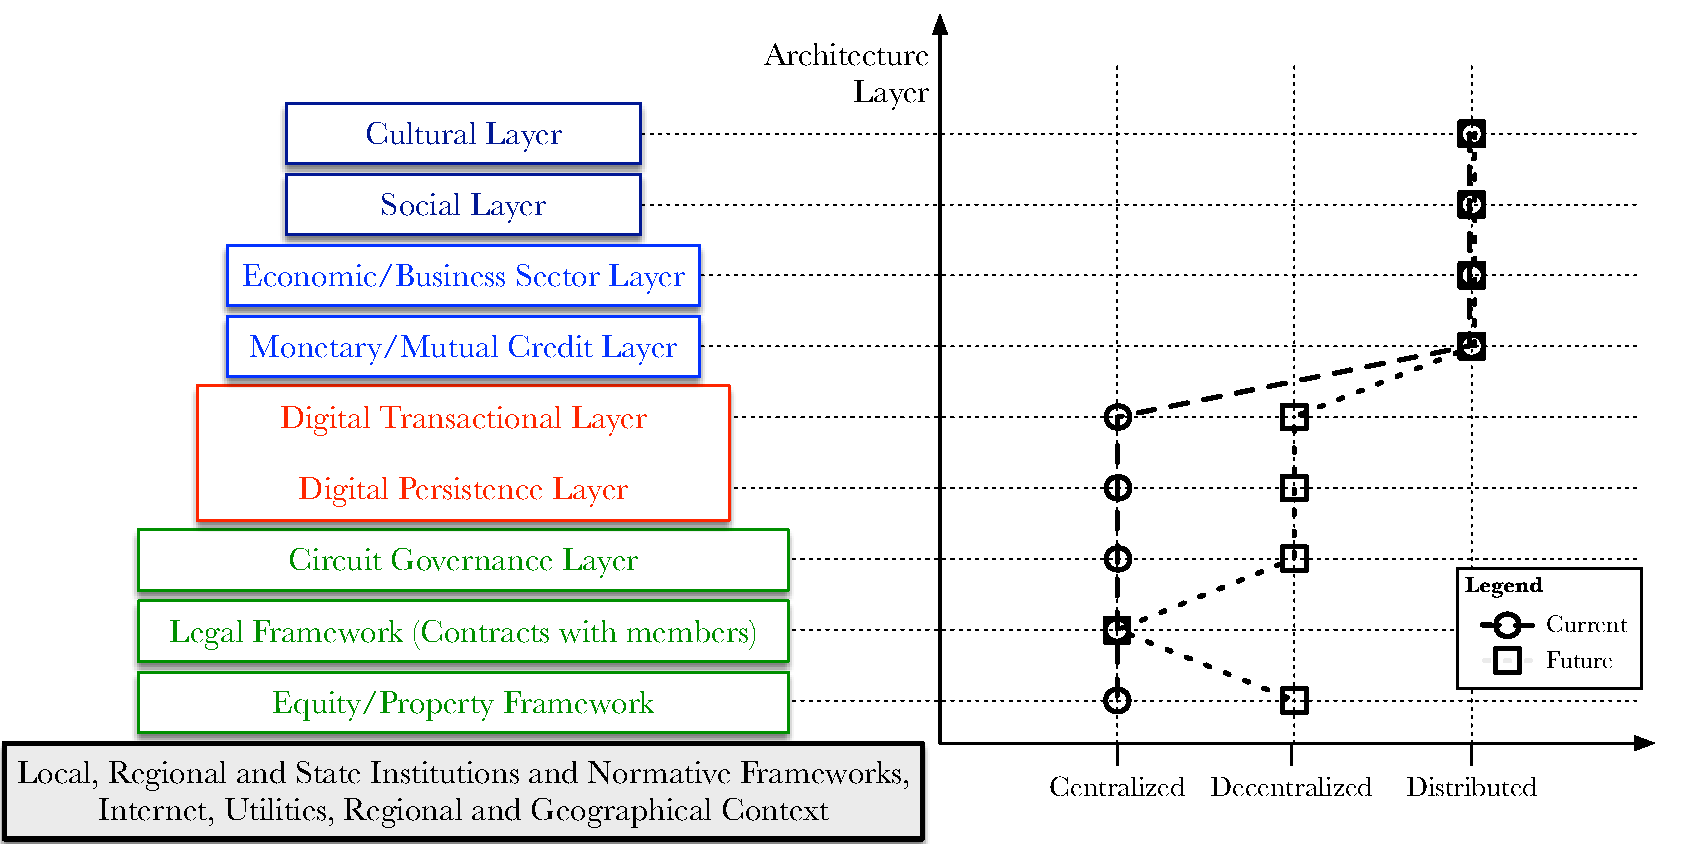
\includegraphics[width=16cm]{Figures/Sardex_Institutional_Structure_V3}
\caption{\small\textbf{Sardex's institutional architecture with current and future decentralization levels}}
\label{decentralizedarchitecture}
\end{figure}

It is too early to imagine what form the fully distributed architecture will take, especially since blockchain technology is being innovated and is diversifying as different forks at incredible speed. Equally important is the principle according to which the technological architecture should be seen as reflecting and responding to the requirements set by the economic, financial, and governance model, and not the other way around. Since the economic, financial, and governance model is also evolving, it is more important to work towards a tight coupling (e.g.\ a compiler) between a formal but agile specification framework and the corresponding implementation than to have all the architectural answers now.

As stated in the Introduction, we are using the ASM method  \cite{BoergerStaerk2003} to develop executable models of the functional requirements. These models will be implemented in the \textbf{coreASIM} framework,\footnote{\url{http://biomicsproject.eu/news/135-icef}} where they can be validated before implementing them in a production environment (e.g.\ in Java).

\subsection{Context and Previous Work}
The INTERLACE proposal describes a blockchain architecture based on the Open Transaction protocol (OTX) \cite{Odom} as an intermediate solution between fully centralized and distributed architectures. OTX involves a pool of Auditor nodes to validate the transactions executed by each Notary node. The initial conception of the INTERLACE architecture was to use only one central Notary, as a first step from the current centralized server towards a more distributed architecture. For the persistence layer we originally examined the Lightweight Cryptocurrency Ledger (LCL) \cite{White2015} as an alternative to the Bitcoin blockchain. The idea of LCL is to store minimal information on the current state of the whole ledger in each block rather than requiring nodes to carry the whole history of block deltas as the Bitcoin blockchain does. This approach achieves continuity with the existing solution while also enabling scalability to multiple circuits (multiple Notaries) under the same mathematical and computational framework.

Rather than replicating the functionality of Cyclos 4 in a decentralized or distributed manner by implementing the OTX-LCL concepts from scratch, it makes sense to take advantage of the staggering levels of investment currently being made in blockchain technologies by several banking and industry consortia, especially since the best ones are open source, and build on existing frameworks. As of April 2017, just before INTERLACE started, the two most likely candidates for our purposes were IBM's Hyperledger Fabric\footnote{\url{https://hyperledger-fabric.readthedocs.io/en/latest/}}\cite{Cachin2016} and Corda.\footnote{\url{https://www.corda.net/}} Together, they can be described as bringing together the principles of OTX and LCL with the smart contracts of Ethereum.\footnote{\url{https://www.ethereum.org/}} However, an important difference is that these blockchain implementations are �permissioned�, they are not open (�permissionless�) like the Bitcoin or Ethereum blockchains. Although this suits the early decentralised implementation of the INTERLACE blockchain, it opens up governance questions that are currently being examined by SARDEX. First among these question is the possibility of establishing two separate legal entities:
\begin{packed_item1}
\item Sardex S.p.A. (SARDEX) will maintain its current ownership structure.
\item A new non-profit legal entity, which we can refer to for now as Circuit Coop, or more loosely as sardex.net, may be formed in the near future to begin devolving the ownership of the commons\footnote{The Sardex circuit commons have not been defined yet, but they will constitute a new basis for shared ownership by all the members. An example could be solar panels owned by the coop and providing renewable energy that can only be bought with credits.} to the circuit members.
\end{packed_item1}

From a purely functional point of view, Hyperledger enables a given node to belong to multiple blockchain networks. This is of interest to us because in the governance framework SARDEX is defining at least two units to be stored on the blockchain are envisaged: SRD credits and a new meritocratic reward points system called `Proximity', implemented with tokens that are earned through altruistic behaviour and dubbed `$\pi$'. Corda is interesting because it separates what Hyperledger calls `chaincode', which implements the smart contracts, from the persistence layer. Thus, Corda comes with a `business flow' layer that provides greater flexibility to adapt to the great diversity of actors in the possible future scenarios, e.g.\ partially overlapping networks involving trade, communications, and renewable energy, and across different regions or even countries.

The functional requirements addressed in this report cover the core functionalities like credit and debit operations but exclude and intentionally hide implementation details about how transactions are actually processed on the backend servers. The reason is to divide the development work into simpler stages rather than achieving the redesign of the full stack in one step. This is thanks to coreASIM acting as an interpreter of executable ASIM models, which can invoke interface object to a simplified user interface and to the backend. In this manner the high-level specification and requirements can be verified before the implementations of either the new front-end and backend are performed.

\subsection{Requirements Overview}\label{_requirements_overview}
The requirements have drifted over time due to two causes. First, the technology is changing very quickly, so what we envisaged in terms of technologies at the time of the proposal writing is now obsolete; second, the governance, economic, and financial model of Sardex is \emph{also} evolving, so the high-level requirements themselves have changed relative to a year ago. Therefore, the requirements below will be instantiated in a specific development strategy to be detailed later in this chapter.
\setcounter{table}{0}
\setlength{\tabcolsep}{10pt}
\begin{table}[htbp]
\begin{centering}
\small
{\begin{tabular}{| l | l | }
\hline
\textbf{Req}	& \textbf{Description} \\
\hline
R1 &Needs a transaction layer and a persistence layer\\
\hline
R2 & Both layers must be extensible and scalable to a (global) distributed architecture, \\
&\hspace{0.5cm}but must start decentralized in their initial (local) implementations\\
\hline
R3 &Should be faster than Bitcoin, so a lightweight ledger (fragmented blockchain) approach is preferred	\\
\hline
R4 &Must be able to support intra-trade and inter-trade between multiple circuits. For example, the \\
&\hspace{0.5cm}different circuits could be: \\
&\hspace{1cm}$\bullet$ different Mutual Credit (MC) circuits (Sardex \& Tibex)\\
&\hspace{1cm}$\bullet$ different types of networks (MC circuit and Renewable Energy (RE) network)\\
\hline
R5 &If possible, reuse existing open source solutions and frameworks, within our own customized\\
&\hspace{0.5cm}ASM/ASIM framework \\
\hline
R6 &Chain code (smart contracts code) should be separate from transaction layer for greater speed\\
&\hspace{0.5cm}and efficiency \\
\hline
R7 &Inter-circuit operations must avoid falling under the European PSD2 Directive\\
\hline
R8 &The Sardex blockchain should not have a native token: this is in order to separate unit of account \\
&\hspace{0.5cm}and medium of exchange from the operation of platform (i.e. no mining, as in Bitcoin) and avoid\\
&\hspace{0.5cm}seignorage (as in Ripple/XRP)	\\
\hline
R9 &Smart contracts code can be Turing-complete. The undecidability of Turing-complete languages does\\
&\hspace{0.5cm}not prevent the ability to prove specific properties of specific programs. In the ASM methodology,\\
&\hspace{0.5cm}provability is refined along with the specifications as part of the iterative refinement process,\\
&\hspace{0.5cm}down to the actual code.\\
\hline
R10 &Industry, Academia, NGO, non-profit, Social Movements\\
\hline
R11 &Platform must involve the current regional MC systems and a reward and digital asset system called\\
&\hspace{0.5cm}Proximity and whose unit of account is called $\pi$\\
\hline
R12 &Proximity involves a reward points system whereby $\pi$s are awarded to users on the basis of\\
&\hspace{0.5cm}behaviour that is beneficial for (their local) MC system. Gaining $\pi$s translates into the ability to\\
&\hspace{0.5cm}trade farther away from the user's geographical location. Upon reaching a certain threshold,\\
&\hspace{0.5cm}the user is allowed to trade inter-circuit.  \\
\hline
R13 &The new platform architecture should be closed, i.e.\ `permissioned', both for the regional networks\\
&\hspace{0.5cm}and for Proximity: Open (permissionless) DLT networks like Ripple/XRP could not prevent\\
&\hspace{0.5cm}external actors from speculating on Sardex digital assets like $\pi$. Private (permissioned) DLTs\\
&\hspace{0.5cm}like Chain Core/Ivy (compatible with PSD2) are preferred \\
\hline
R14 &State objects must be immutable: this is important in order to prevent people going back on their\\
&\hspace{0.5cm}commitments, for example the max number of credits they will accept (there are examples of\\
&\hspace{0.5cm}blockchains whose previous blocks have been modified, such as the Ethereum DAO Hack)  \\
\hline
\end{tabular}}
\caption{\small\textbf{Summary of initial high-level requirements}}
\label{ReqTable}
\end{centering}
\end{table}

\subsection{Quality Goals}\label{_quality_goals}

\subsection{Stakeholders and their roles}\label{_stakeholders}

\begin{itemize}
	\item B ... Business
	\item C ... Customer
	\item E ... Employee	
\end{itemize}

\begin{longtable}[]{@{}lll@{}}
\toprule
\begin{minipage}[b]{0.18\columnwidth}\raggedright\strut
Role/Name\strut
\end{minipage} & \begin{minipage}[b]{0.37\columnwidth}\raggedright\strut
Contact\strut
\end{minipage} & \begin{minipage}[b]{0.37\columnwidth}\raggedright\strut
Expectations\strut
\end{minipage}\tabularnewline
\midrule
\endhead
\begin{minipage}[t]{0.18\columnwidth}B2B \end{minipage} &
\begin{minipage}[t]{0.37\columnwidth}Participating Companies \end{minipage} &
\begin{minipage}[t]{0.37\columnwidth}Business to business transactions and interaction\end{minipage}
\tabularnewline
\tabularnewline
\begin{minipage}[t]{0.18\columnwidth}B2E \end{minipage} &
\begin{minipage}[t]{0.37\columnwidth}Employees \end{minipage} &
\begin{minipage}[t]{0.37\columnwidth}Payments of Employees\end{minipage}
\tabularnewline
\tabularnewline
\begin{minipage}[t]{0.18\columnwidth}B2C \end{minipage} &
\begin{minipage}[t]{0.37\columnwidth}Normal Customer \end{minipage} &
\begin{minipage}[t]{0.37\columnwidth}Payments to Participating Companies\end{minipage}
\tabularnewline
\tabularnewline
\begin{minipage}[t]{0.18\columnwidth}Sardex-Admin \end{minipage} &
\begin{minipage}[t]{0.37\columnwidth}Sardex Employee \end{minipage} &
\begin{minipage}[t]{0.37\columnwidth}Configuring and maintaining the infrastructure\end{minipage}
\tabularnewline
\tabularnewline
\begin{minipage}[t]{0.18\columnwidth}Sardex-Manager \end{minipage} &
\begin{minipage}[t]{0.37\columnwidth}Sardex Employee \end{minipage} &
\begin{minipage}[t]{0.37\columnwidth}Running evaluations and managing the cooperation platform \end{minipage}
\tabularnewline


\bottomrule
\end{longtable}

\section{Solution Strategy}\label{section-solution-strategy}
The strategy of how to get from a monolithic working implementation to a decentralized and later a fully distributed ledger application is broken down in several steps, as outlined below.

Since the original ASMs work only in their own scope, it is not possible to create a decentralized or fully distributed environment with them. The solution for the INTERLACE project has been to use a special extension of the ASMs named Abstract Interaction Machines (ASIMs) developed by the BIOMICS project, and a corresponding runtime environment called Interaction Computing Execution Framework (ICEF) \footnote{\url{https://github.com/biomics/icef}}. As explained on the ICEF webpage:
\begin{quote}
\vspace{-0.3cm}
This framework extends the original CoreASM modelling and execution framework to enable the specification and execution of \textbf{distributed and concurrent} ASMs. The ICEF was developed in the STREP project BIOMICS which was financed by the European Comission in FP7 from October 1st, 2012 until March 31st, 2016. ICEF enables asynchronous execution of ASMs. It uses and enhances the CoreASM execution engine to support communicating and interacting ASMs: CoreASIMs. Further, ICEF replaces ASM with BSL which offers additional language primitives specifically designed to define the beahviour of biochemical systems. This code introduces a restful API to control the BIOMICS wrapper (brapper) which can host several CoreASIM instances and enables networked CoreASIM. It also introduces a manager which orchestrates several ASIMs to allow the execution of interaction computing simulations.
\end{quote}

Although the additional language primitives offered by ICEF might not be needed, the coreASIM implementation will be crucial for realizing the INTERLACE strategy.

\subsection{Strategy Steps}\label{subsection-strategy-steps}

\begin{enumerate}
	\item Define the functional requirements of the business logic using the ASMs formal description language (this report).
	\item Translate the formal description to a working demo environment using ICEF/coreASIM.
	\item Connect the business logic modelled with ASMs and implemented in coreASIM to the real world. That means use the interaction capabilities of the framework to connect it to the existing legacy application used by SARDEX, Cyclos 4. This existing working architecture is summarized at a high level in Figure \ref{cyclosarchitecture}.
	\item Test if the application and the translation to coreASIM work.
	\item Translate the coreASIM implementation to a real-world application by creating e.g.\ a JAVA. application.
	\item Develop a verification strategy and validate the implemented real-world application through component testing.
	\item Select appropriate blockchain technologies for the next-generation infrastructure.
	\item Develop ASIM specifications that model the distributed environment.
	\item Adapt ASIM interfaces.
	\item Adapt the real-world version of the application to the new infrastructure.
	\item Implement the new back-end logic using Open Source frameworks.
	\item Test/Validate with real users the new application against the new back-end.
\end{enumerate}


\begin{figure}[htbp]
\centering
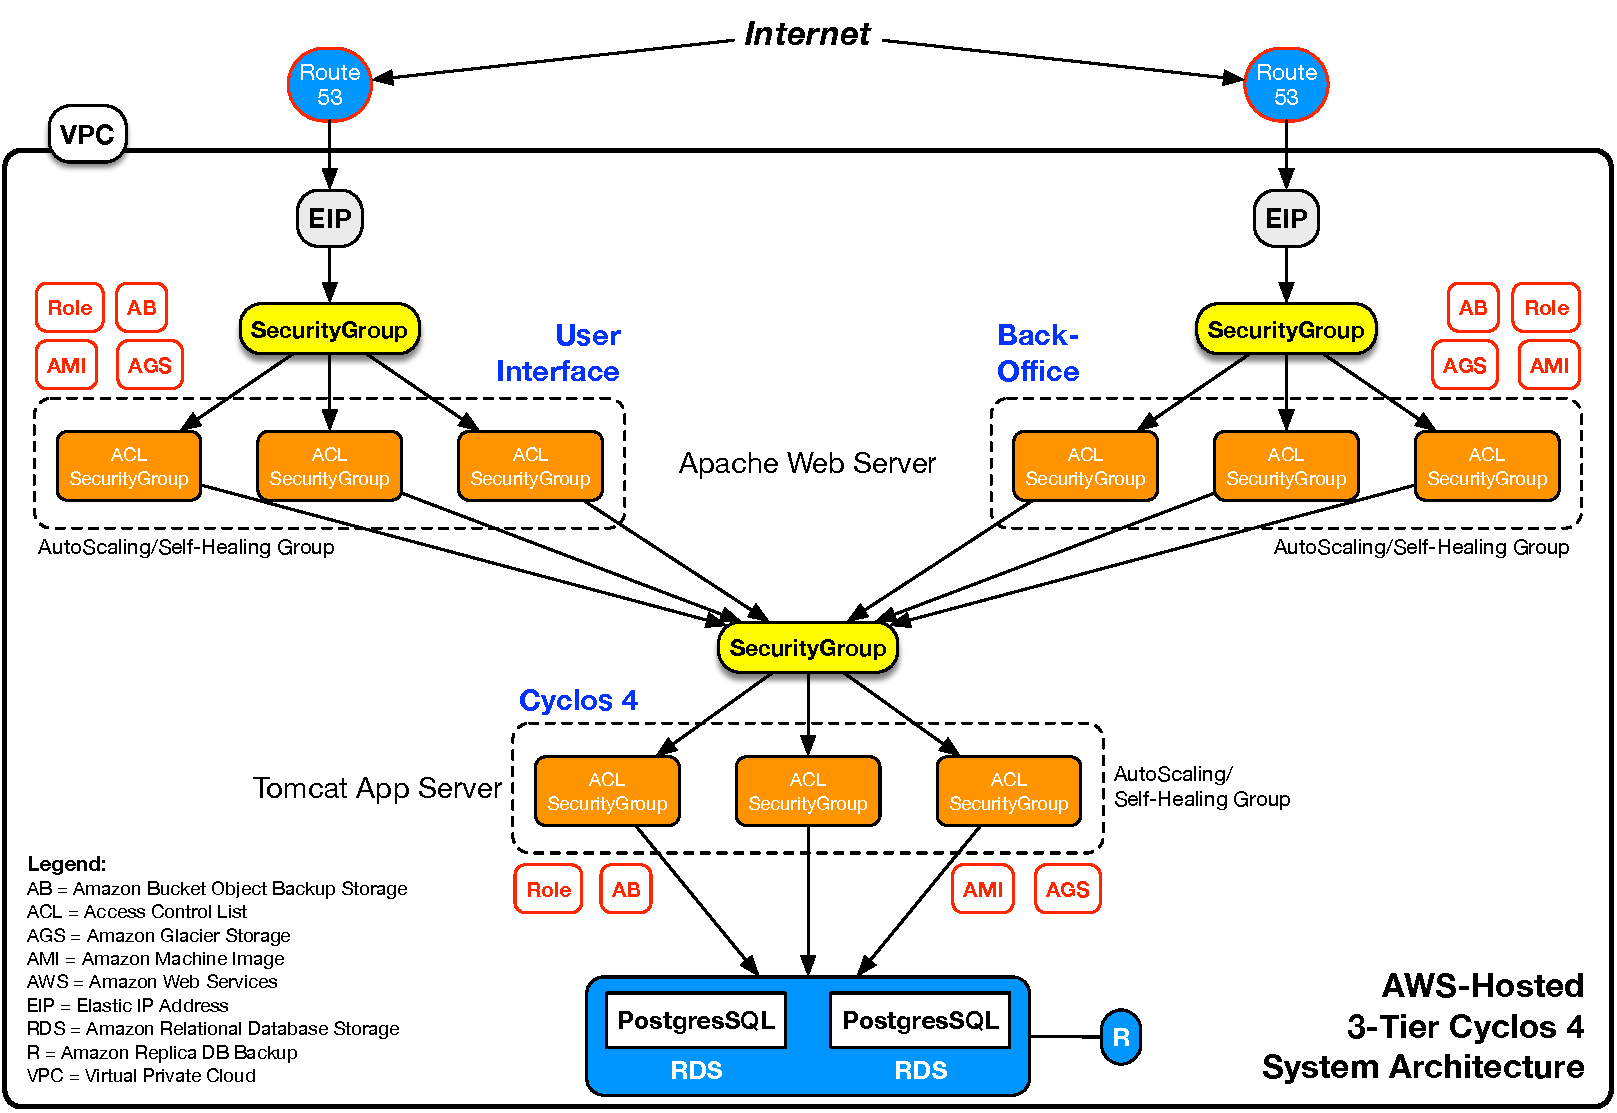
\includegraphics[width=17.5cm]{Figures/3-Tier_Cyclos_Architecture}
\caption{\small\textbf{Existing 3-tier Cyclos 4 architecture used by SARDEX, based on Amazon Web Services}}
\label{cyclosarchitecture}
\end{figure}




%\section{Architecture
%Constraints}\label{section-architecture-constraints}

%\section{System Scope and
%Context}\label{section-system-scope-and-context}

%\subsection{Business Context}\label{_business_context}

%\textbf{\textless{}Diagram or Table\textgreater{}}

%\textbf{\textless{}optionally: Explanation of external domain
%interfaces\textgreater{}}

%\subsection{Technical Context}\label{_technical_context}

%\textbf{\textless{}Diagram or Table\textgreater{}}

%\textbf{\textless{}optionally: Explanation of technical
%interfaces\textgreater{}}

%\textbf{\textless{}Mapping Input/Output to Channels\textgreater{}}

%\section{Solution Strategy}\label{section-solution-strategy}

%\section{Building Block View}\label{section-building-block-view}

%\subsection{Whitebox Overall System}\label{_whitebox_overall_system}

%\emph{\textbf{\textless{}Overview Diagram\textgreater{}}}

%\begin{description}
%\item[Motivation]
%\emph{\textless{}text explanation\textgreater{}}
%\item[Contained Building Blocks]
%\emph{\textless{}Description of contained building block (black
%boxes)\textgreater{}}
%\item[Important Interfaces]
%\emph{\textless{}Description of important interfaces\textgreater{}}
%\end{description}

%\subsubsection{\textless{}Name black box
%1\textgreater{}}\label{__name_black_box_1}

%\emph{\textless{}Purpose/Responsibility\textgreater{}}

%\emph{\textless{}Interface(s)\textgreater{}}

%\emph{\textless{}(Optional) Quality/Performance
%Characteristics\textgreater{}}

%\emph{\textless{}(Optional) Directory/File Location\textgreater{}}

%\emph{\textless{}(Optional) Fulfilled Requirements\textgreater{}}

%\emph{\textless{}(optional) Open Issues/Problems/Risks\textgreater{}}

%\subsubsection{\textless{}Name black box
%2\textgreater{}}\label{__name_black_box_2}

%\emph{\textless{}black box template\textgreater{}}

%\subsubsection{\textless{}Name black box
%n\textgreater{}}\label{__name_black_box_n}

%\emph{\textless{}black box template\textgreater{}}

%\subsubsection{\textless{}Name interface
%1\textgreater{}}\label{__name_interface_1}

%\ldots{}

%\subsubsection{\textless{}Name interface
%m\textgreater{}}\label{__name_interface_m}

%\subsection{Level 2}\label{_level_2}

%\subsubsection{\texorpdfstring{White Box \emph{\textless{}building block
%1\textgreater{}}}{White Box \textless{}building block 1\textgreater{}}}\label{_white_box_emphasis_building_block_1_emphasis}

%\emph{\textless{}white box template\textgreater{}}

%\subsubsection{\texorpdfstring{White Box \emph{\textless{}building block
%2\textgreater{}}}{White Box \textless{}building block 2\textgreater{}}}\label{_white_box_emphasis_building_block_2_emphasis}

%\emph{\textless{}white box template\textgreater{}}

%\ldots{}

%\subsubsection{\texorpdfstring{White Box \emph{\textless{}building block
%m\textgreater{}}}{White Box \textless{}building block m\textgreater{}}}\label{_white_box_emphasis_building_block_m_emphasis}

%\emph{\textless{}white box template\textgreater{}}

%\subsection{Level 3}\label{_level_3}

%\subsubsection{White Box \textless{}\_building block
%x.1\_\textgreater{}}\label{_white_box_building_block_x_1}

%\emph{\textless{}white box template\textgreater{}}

%\subsubsection{White Box \textless{}\_building block
%x.2\_\textgreater{}}\label{_white_box_building_block_x_2}

%\emph{\textless{}white box template\textgreater{}}

%\subsubsection{White Box \textless{}\_building block
%y.1\_\textgreater{}}\label{_white_box_building_block_y_1}

%\emph{\textless{}white box template\textgreater{}}

%\section{Runtime View}\label{section-runtime-view}

%\subsection{\textless{}Runtime Scenario
%1\textgreater{}}\label{__runtime_scenario_1}

%\begin{itemize}
%\item
%  \emph{\textless{}insert runtime diagram or textual description of the
%  scenario\textgreater{}}
%\item
%  \emph{\textless{}insert description of the notable aspects of the
%  interactions between the building block instances depicted in this
%  diagram.\textgreater{}}
%\end{itemize}

%\subsection{\textless{}Runtime Scenario
%2\textgreater{}}\label{__runtime_scenario_2}

%\subsection{\ldots{}}\label{_}

%\subsection{\textless{}Runtime Scenario
%n\textgreater{}}\label{__runtime_scenario_n}

%\section{Deployment View}\label{section-deployment-view}

%\subsection{Infrastructure Level 1}\label{_infrastructure_level_1}

%\emph{\textbf{\textless{}Overview Diagram\textgreater{}}}

%\begin{description}
%\item[Motivation]
%\emph{\textless{}explanation in text form\textgreater{}}
%\item[Quality and/or Performance Features]
%\emph{\textless{}explanation in text form\textgreater{}}
%\item[Mapping of Building Blocks to Infrastructure]
%\emph{\textless{}description of the mapping\textgreater{}}
%\end{description}

%\subsection{Infrastructure Level 2}\label{_infrastructure_level_2}

%\subsubsection{\texorpdfstring{\emph{\textless{}Infrastructure Element
%1\textgreater{}}}{\textless{}Infrastructure Element 1\textgreater{}}}\label{__emphasis_infrastructure_element_1_emphasis}

%\emph{\textless{}diagram + explanation\textgreater{}}

%\subsubsection{\texorpdfstring{\emph{\textless{}Infrastructure Element
%2\textgreater{}}}{\textless{}Infrastructure Element 2\textgreater{}}}\label{__emphasis_infrastructure_element_2_emphasis}

%\emph{\textless{}diagram + explanation\textgreater{}}

%\ldots{}

%\subsubsection{\texorpdfstring{\emph{\textless{}Infrastructure Element
%n\textgreater{}}}{\textless{}Infrastructure Element n\textgreater{}}}\label{__emphasis_infrastructure_element_n_emphasis}

%\emph{\textless{}diagram + explanation\textgreater{}}

%\section{Cross-cutting Concepts}\label{section-concepts}

%\subsection{\texorpdfstring{\emph{\textless{}Concept
%1\textgreater{}}}{\textless{}Concept 1\textgreater{}}}\label{__emphasis_concept_1_emphasis}

%\emph{\textless{}explanation\textgreater{}}

%\subsection{\texorpdfstring{\emph{\textless{}Concept
%2\textgreater{}}}{\textless{}Concept 2\textgreater{}}}\label{__emphasis_concept_2_emphasis}

%\emph{\textless{}explanation\textgreater{}}

%\ldots{}

%\subsection{\texorpdfstring{\emph{\textless{}Concept
%n\textgreater{}}}{\textless{}Concept n\textgreater{}}}\label{__emphasis_concept_n_emphasis}

%\emph{\textless{}explanation\textgreater{}}

%\section{Design Decisions}\label{section-design-decisions}

%\section{Quality Requirements}\label{section-quality-scenarios}

%\subsection{Quality Tree}\label{_quality_tree}

%\subsection{Quality Scenarios}\label{_quality_scenarios}

\section{Risks and Technical Debts}\label{section-technical-risks}

\section{Glossary}\label{section-glossary}

\begin{longtable}[]{@{}ll@{}}
\toprule
\begin{minipage}[b]{0.47\columnwidth}\raggedright\strut
Term\strut
\end{minipage} & \begin{minipage}[b]{0.47\columnwidth}\raggedright\strut
Definition\strut
\end{minipage}\tabularnewline
\midrule
\endhead
\begin{minipage}[t]{0.47\columnwidth}\raggedright\strut
\textless{}Term-1\textgreater{}\strut
\end{minipage} & \begin{minipage}[t]{0.47\columnwidth}\raggedright\strut
\textless{}definition-1\textgreater{}\strut
\end{minipage}\tabularnewline
\begin{minipage}[t]{0.47\columnwidth}\raggedright\strut
\textless{}Term-2\textgreater{}\strut
\end{minipage} & \begin{minipage}[t]{0.47\columnwidth}\raggedright\strut
\textless{}definition-2\textgreater{}\strut
\end{minipage}\tabularnewline
\bottomrule
\end{longtable}
